\documentclass[runningheads]{llncs}

\usepackage{graphicx}
\usepackage{todonotes}
\usepackage{listingsutf8}
\usepackage[hidelinks]{hyperref}
\usepackage{cleveref}
\usepackage{footmisc}
\usepackage{bookmark}

\renewcommand\UrlFont{\color{blue}\rmfamily}

\begin{document}

\title{CaRSA Data Identify, Collect, and Connect: A second-generation, national GeoLD system in Australia}
\titlerunning{CaRSA LocI}

\author{
    Nicholas J. Car\inst{1}\orcidID{0000-0002-8742-7730} \and \\
    Irina Bastrakova\inst{2}\orcidID{0000-0002-4643-7289}
}

\authorrunning{Car N.J. et al.}

\institute{
    {
    SURROUND Australia Pty Ltd., Australia \&\\
    Australian National University, Australia\\
    \email{nicholas.car@surroundaustralia.com}
    %\url{https://surroundaustralia.com}
    }
    \and
    {
        Geoscience Australia\\
        \email{irina.bastrakova@ga.gov.au}
    }
}

\maketitle

\begin{abstract}
In 2018 – 2020, Australia built two \textit{Linked Data} ``spines'' - themed collections of interoperable reference data - called LocI and LongSpine. 
LocI (Location Index) consists of 7 nationally-significant spatial datasets such as the Australian Statistical Geographies System. 
LongSpine (Longitudinal Spine of Government Functions) consists of multiple datasets of Australian government structure. Both projects interpreted existing open 
datasets into Linked Data form and provided online delivery of their the parts as well as infrastructure for their use as a single system.\\

Here described is the Climate and Resilience Services Australia’s Data Identify, Collect and Connect project's reuse and extension of LocI. 
We discuss LocI design, this project's differences and key requirement of this project, in particular the requirement to work with non-Linked Data 
spatial data systems, and how this system is pushing spatial and \textit{Semantic Web} standards development such as DGGS and GeoSPARQL.

\keywords{Location Index \and LocI \and GeoSPARQL \and DGGS \and Spatial Data on the Web \and Australia \and national data infrastructure}
\end{abstract}


\section{Introduction}\label{sec:introduction}
\subsection{CaRSA Motivation}
Climate and Resilience Services Australia (CaRSA) is a new Australia government cross-agency initiative\footnote{``Australia commits to climate resilience'', \url{https://minister.awe.gov.au/ley/media-releases/australia-commits-climate-resilience}}
that will:

\begin{quote}
    connect and leverage the Commonwealth’s extensive climate and natural disaster risk information to further prepare for and build 
    resilience to natural disasters
\end{quote}

Since Australia is prone to very damaging natural disasters such as bush fires, floods and droughts, this is a major government initiative
allocated good resourcing and the commitment is for multiple years.

\subsection{CaRSA Demonstrator Projects}
Several of the demonstrator projects for CaRSA sought to test different ways of combining information from multiple government agencies 
relevant to natural disaster management. Traditional methods of data aggregation are being tested, such as data pooling in shared facilities,
standardiseing web service-delivered information and cross-cataloging datasets, but forward-looking methdos are too. In particular,
\textit{Semantic Web} (SW) and \textit{Linked Data} (LD) technologies\footnote{By ``Linked Data'', as opposed to ``linked data'' or ``data linkage'' etc.,
we mean systems and data that implement a number of \textit{Semantic Web} technologies (RDF, OWL, SKOS, SPARQL, etc.) which are primarily 
defined as a series of \href{https://www.w3.org/standards/semanticweb/data}{World Wide Web Consortium} (W3C) standards. The W3C's defintion of 
\textit{Semantic Web} is that it is a ``Web of Data'', an evolved Internet able to be queried by machineswhich can draw inferences from it.}
are being used to integrate different, but relativley similar, datasets that are published in a distributed manner and
\textit{Discrete Global Grid System} (DGGS) spatial data methods are being used to integrate spatial data from multiple sources.

This paper describes the SW/LD and DGGS approaches being implemented in CaRSA's ``Data Identify, Collect, and Connect'' project that we will 
refere to as \textit{this project}. The project extends the approach taken by the Location Index project described in the next section.

\section{LocI: The Loction Index}\label{sec:loci}

\begin{figure}[htb]
    \centering
    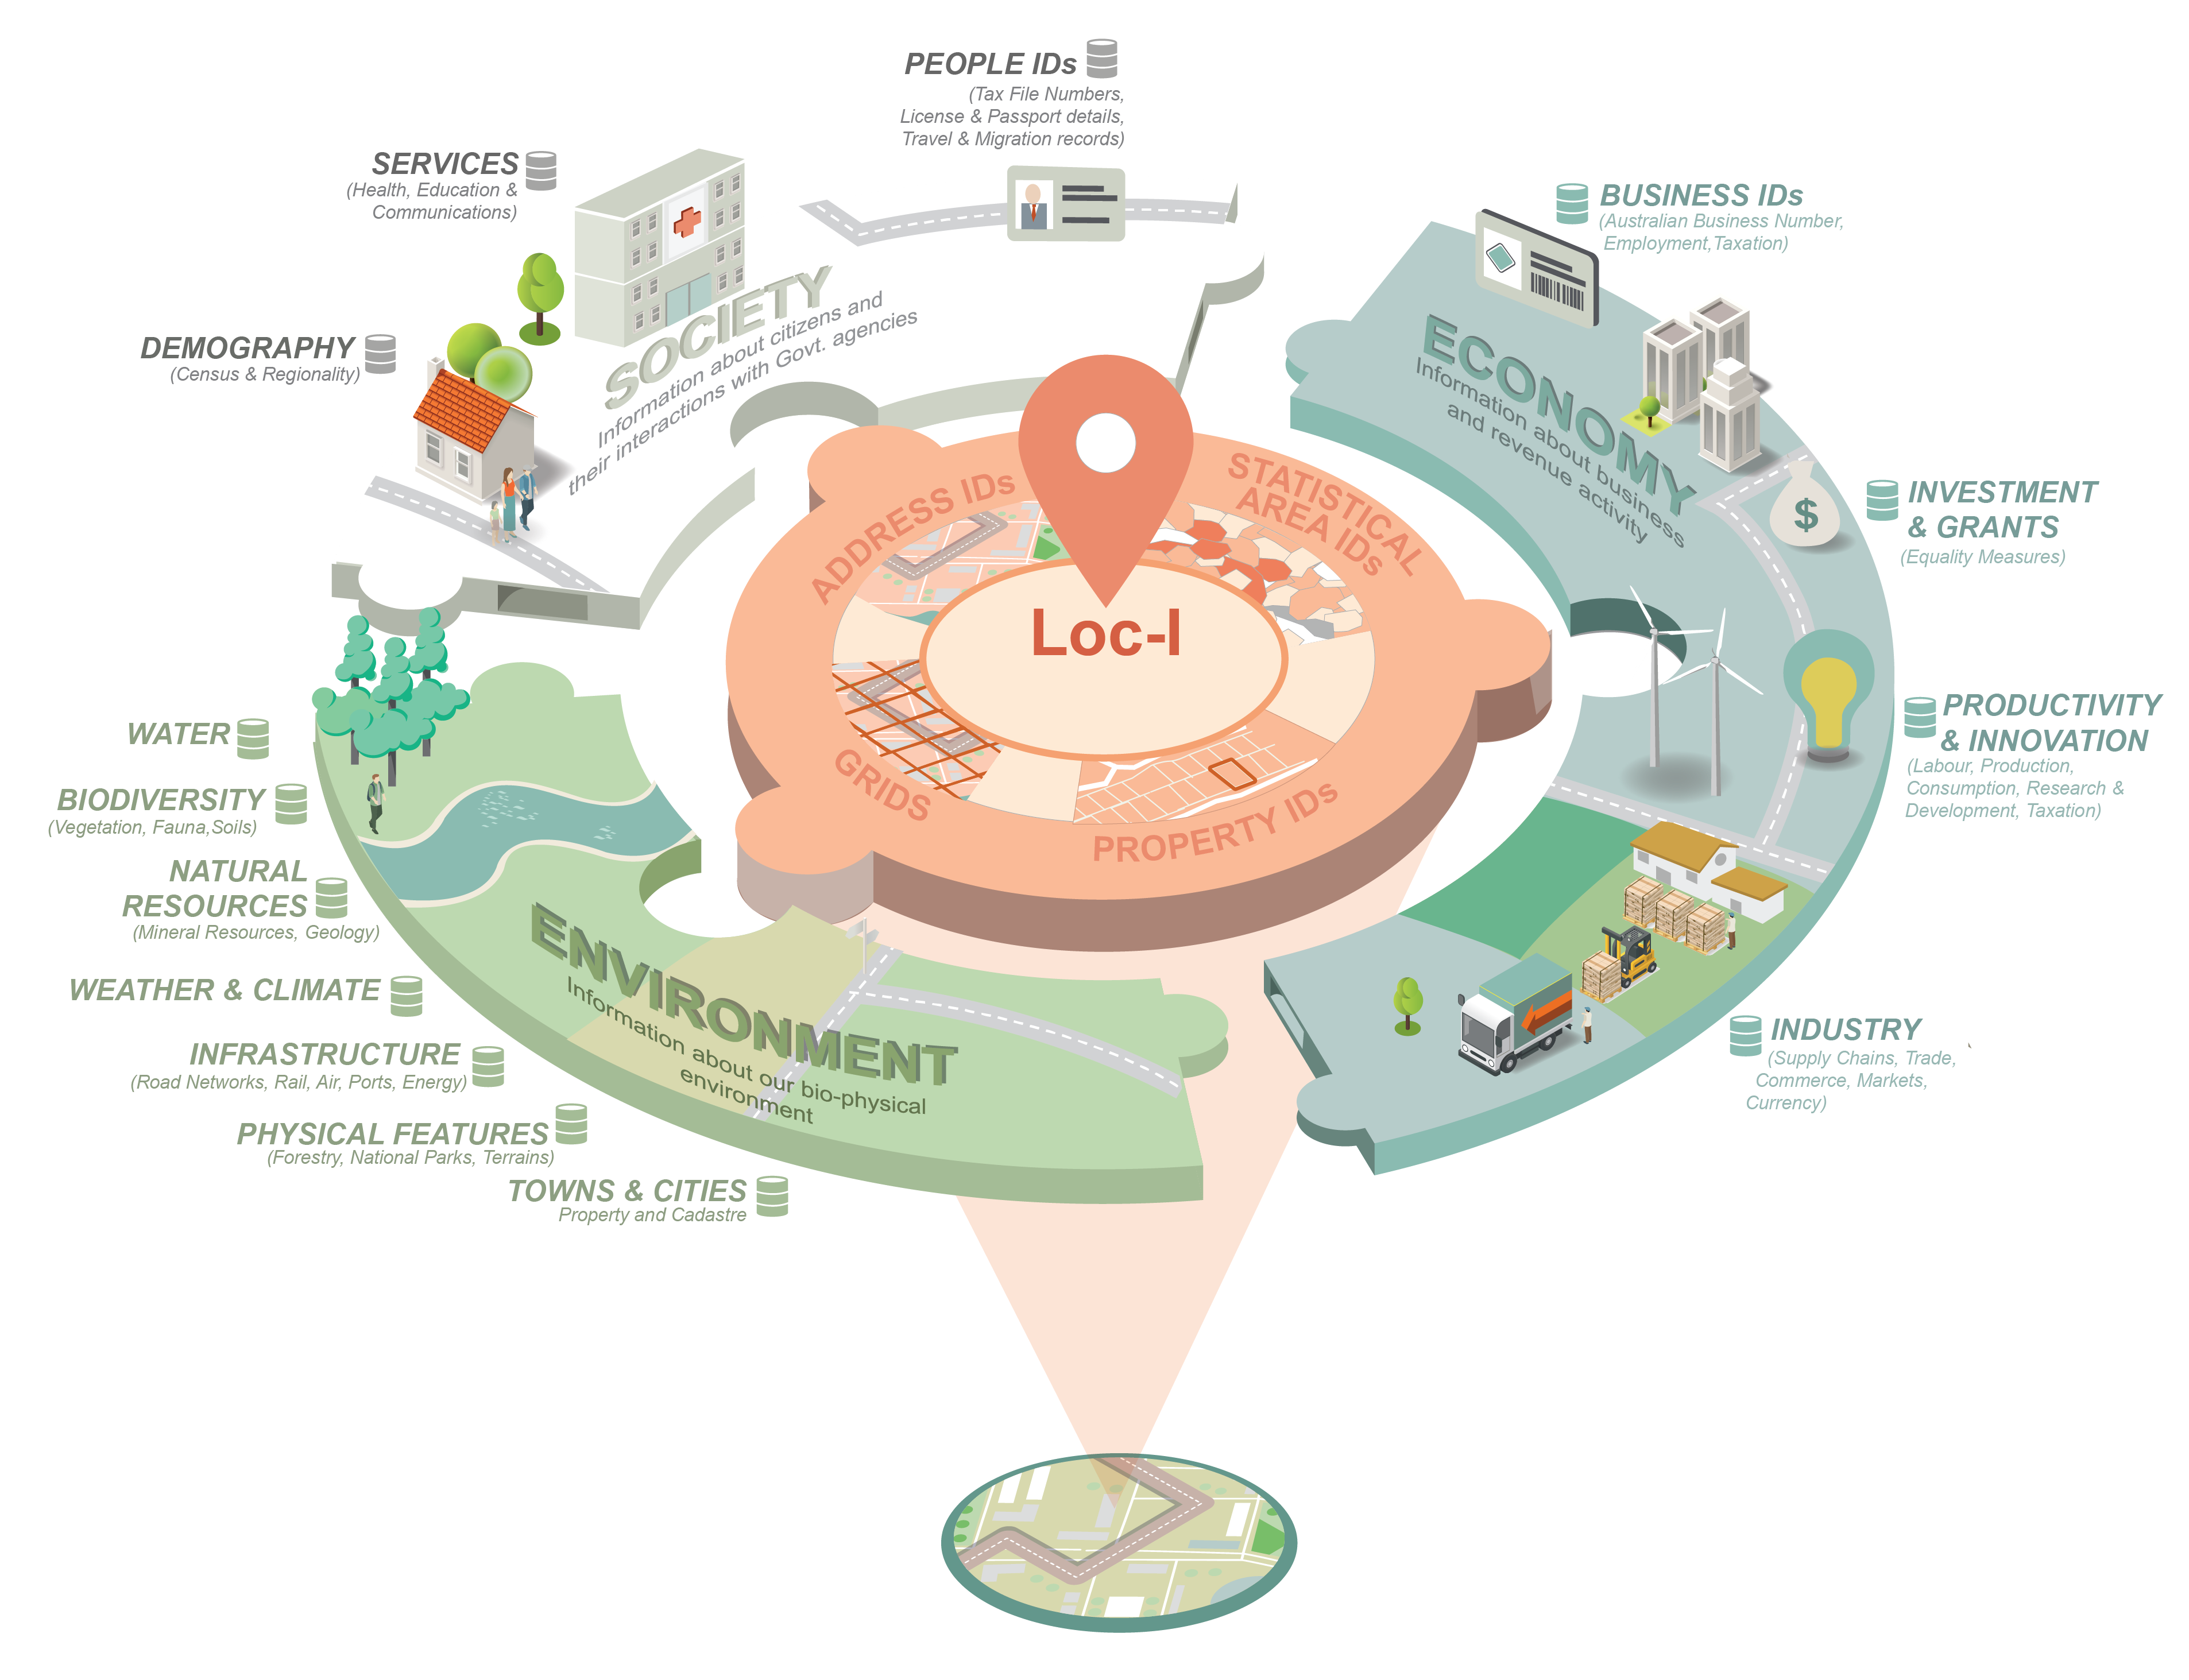
\includegraphics[width=\linewidth]{images/loci-brochure.png}
    \caption{A project brochure image, from \cite{car_location_2019}, of LocI with respect to
    Australian government \textit{Environment}, \textit{Society} and \textit{Economy} data}
    \label{fig:loci-brochure}
\end{figure}

In 2018 - 2020, Australian spatial data and research agencies implemented a:

\begin{quotation}
    national and authoritative, also federated, index for Australian spatial data using Semantic Web technologies~\cite{car_location_2019}
\end{quotation}

This system, known as the Location Index (LocI)~\cite{car_location_2019}, aims to ``better geospatially integrate and analyze data across 
government portfolios and information domains''. The main use case addressed by LocI's is to greatly reduce the time taken by government 
workers in data analysis using spatial information by providing pre-integrated, authoratitive, spatial datasets that can be used in 
online, open data scenarios, within secure data integration environments and across the two. The project deals with data from multiple domains,
see Figure~\ref{fig:loci-brochure}.

Some of the interesting aspects of LocI's design include:

\begin{itemize}
    \item[$\ast$] federated publication of datasets via standard Linked Data APIs
    \item[$\ast$] use of VoID \texttt{Linkset}~\footnote{\url{https://www.w3.org/TR/void/}} instances to crosswalk datasets
    \begin{itemize}
        \item[$-$] these are independently-selectable for use meaning that a specific ccrosswalk, of potentially many, may be selected for use
    \end{itemize} 
    \item[$\ast$] use of a \textit{Geometry Data Service}\footnote{The service is online at \url{https://gds.loci.cat/}} for spatial integration
    \begin{itemize}
        \item[$-$] this service extends common use of using GeoSPARQL~\cite{open2012ogc} by storing \texttt{Geometry} instances seperately from the \texttt{Feature} instances they are the geometries for. This allows the geometry data to be managed in a PostGIS database~\footnote{\url{https://postgis.net/}}, not a triplestore, as usually used for GeoSPARQL data.
    \end{itemize}
    \item[$\ast$] several different clients for different uses
    \begin{itemize}
        \item[$-$] such as \textit{Excelerator}\footnote{\url{https://loci.cat/excelerator.html}}, used to upload data according to one spatial reference system and download it reapportioned according to another
    \end{itemize}
\end{itemize} 

LocI's datasets are from many domains including environmental (the \textit{Australian Hydrological Geospatial Fabric}
\footnote{Original, non-RDF dataset: \url{http://www.bom.gov.au/water/geofabric/}, and the online LD version implemented by LocI: \url{http://linked.data.gov.au/dataset/geofabric}}, 
a collection of surface hydrology features), human/census (the \textit{Australian Statistical Geography Standard} spatial areas)
\footnote{Non-RDF dataset: \url{https://geo.abs.gov.au/arcgis/services/ASGS2016/MB/MapServer/WFSServer}, LD version: \url{http://linked.data.gov.au/dataset/asgs2016}}, 
and cartographic/administrative (the \textit{National Composite Gazetteer of Australia})\footnote{LD version: \url{https://linked.data.gov.au/dataset/placenames}}. 

LocI architecture is shown in Figure~\ref{fig:loci-arch} for architectural details. It shows the LocI Data Cache, which is a multi-graph triplestore, 
obtains its data by ``pulling'' RDF datasets through APIs that both interpret non-RDF data for online delivery and are also able to create static RDF 
versions of the datasets. All LocI datasets conform to the LocI Ontology\footnote{\url{http://linked.data.gov.au/def/loci}} which imports the GeoSPARQL
\footnote{\url{http://www.opengis.net/doc/IS/geosparql/1.0}} and DCAT\footnote{\url{https://www.w3.org/TR/2014/REC-vocab-dcat-20140116/}} ontologies. 
Alongside the Cache is a traditional spatial DB - PostGIS\footnote{\url{https://postgis.net/}} used to perform fast geometry intersections.

\begin{figure}[htb]
    \centering
    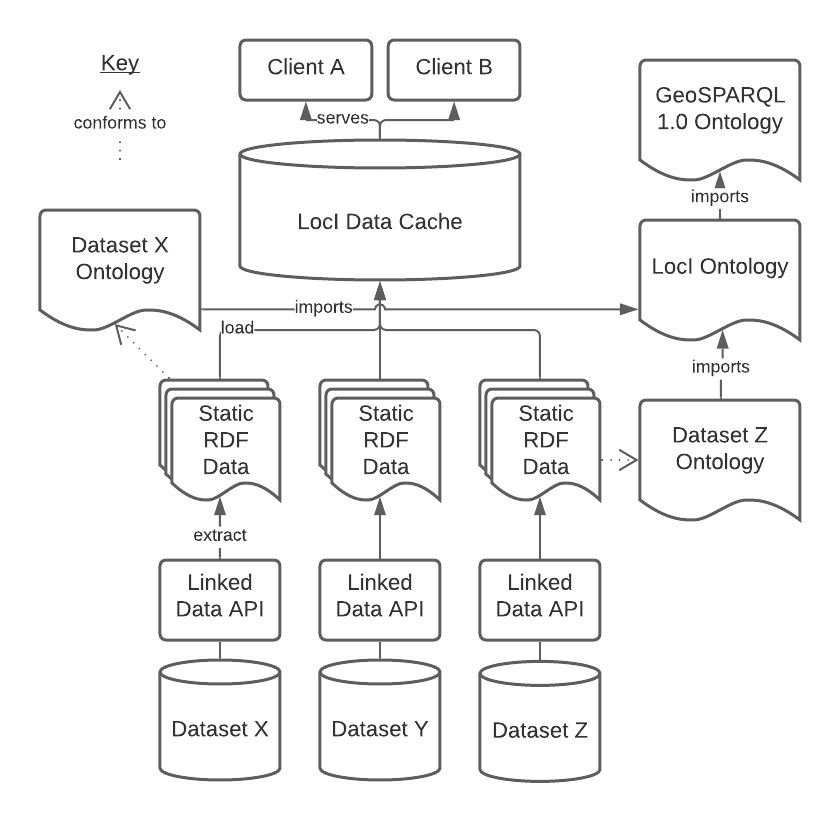
\includegraphics[width=0.8\linewidth]{images/loci-arch.png}
    \caption{An informal architecture diagram of LocI's \textit{Linked Data} infrastructure.}
    \label{fig:loci-arch}
\end{figure}

\section{CaRSA Project Changes}\label{sec:changes}
\subsection{Data Validity}
This project's datasets are LocI datasets and the project knowledge Graph (KG) is similar to the LocI cache, however conformance to LocI is not easily
 testable: data reasoning with LocI ontologies can check for incorrect inferences but no contraint language validators are available. This project implements formal \textit{profiles}, which 
are specifications defining dependencies and validation tooling. This project uses profiles for requirements for data 
publication by API, dataset suitability for the KG and for use and display by clients and they are defined using 
\textit{The Profiles Vocabulary}~\cite{atkinson_profiles_2020} and all listed in the project catalogue\footnote{\label{catalogue} \url{https://w3id.org/carsa-loci/catalogue}}.

\subsection{Discrete Global Grid System (DGGS) use}
LocI aspired to use DGGS geometries\footnote{See the defining \textit{Abstract Specification}~\cite{purss_topic_2017} for indications of potential benefits of 
DGGS and the more recent \textit{OGC Engineering Report}~\cite{gibb_ogc_2021} for current thinking about how to integrate DGGS use within traditional spatial 
infrastructure.} but never really did: DGGS data was produced but not really used. This project has produced DGGS versions of all \texttt{Feature} instances' 
geometries, has stored them alongside traditional geometries within the KG (a triplestore) and has implemented GeoSPARQL~\cite{open2012ogc} functions
within the triplestore SPARQL extension libraries (Apache Jena's ARC\footnote{\url{https://jena.apache.org/documentation/query/extension.html}}) that work with 
DGGS geometry representations. These functions are used to obviate the need for LocI's Geometry Data Store and thus reduce infrastructure complexity.

An important enabling factor in this use of DGGS with GeoSPARQL is the inclusion of DGGS geometry serializations within version 1.1 of GeoSPARQL which was motivated
by LocI project requirements. This version is currently under review and is expected to be published around the time of this paper's publication. Working documents 
are avalable\footnote{See \url{https://opengeospatial.github.io/ogc-geosparql/} for the GeoSPARQL ``Standards Working Groups`` 's working documents}.

\subsection{Observations data use}
LocI anticipated observational data - human/industry statistics or natural-world observation data - wuold be used with its spatial data. This project
implements two such datasets: 1. population data taken from the 2016 Australian census; 2. ``exposure'' data per statistical area - this is data about the vulnerability
of physical infrastructure to natural hazards. This project has developed an ``Observations Dataset'' profile (see the project catalogue \footref{catalogue}) that defines the characteristics of a LocI-comatable 
observations dataset using the profiling mechanisms mentioned above.

\subsection{Knowledge Graph (KG) importing}
This project's KG includes LocI datasets as well as new LocI-conformant datasets. To avoid duplication, this project intends to import LocI content unchanged however, 
currently, the additional requirements this project has (see the listed changes above) mean that LocI datasets have to be extended and thus reuse of LocI datasets
or the data cache (see Figure~\ref{fig:loci-arch}) is not currently possible. For now, a ``LocI 2 KG'' has een created and imported into this project's KG (see 
\ref{fig:carsa-arch}) but this will be removed when LocI implements this project's elements.

\subsection{Clients and Management}
LocI implemented some generic and specific clients of its data holdings\footnote(See \url{https://loci.cat/#datasets-and-applications} for a list). This project can reuse 
some of them, such as \textit{IDer Down}\footnote{\url{https://excelerator.loci.cat/iderdown}} due to the same dataset structures used, however this project has a pair of 
major objectived that have necessitated different clients. These are:

\begin{enumerate}
    \item Management of data by versions in the project KG
    \item Demonstration of the integration of traditional spatial web data display and Linked Data
\end{enumerate} 

For the first, this project has implemented a sophsticated application layer on top of its KG: the \textit{SURROUND Ontology Platform}\footnote{\url{https://surroundaustralia.com/sop}}
is used to track, select for use, update and generally govern datasets. This results in a new administrative interface that LocI never had since it was not tasked with operational
data management, only proof-of-concpet system implementation. For the second, information
flows between a traditional web spatial data portal\footnote{The re-deployable TerriaJS (\url{https://terria.io/}) globe is deployed for this project at \url{https://w3id.org/carsa-loci/globe}}
and a Linked Data browser\footnote{This system allows for the browsing of content within this project's KG, as opposed to the LD dereferencing of individual resources 
which is acomplished by the APIs implemented for each dataset.} with panels of per-\texttt{Feature} information witin the portal supplied by KG queries. This demonstrated
LD / SW data for previous implementations of this data portal software just present simple type key / value pairs of information per-\texttt{Feature}.

\subsection{More standardized Dataset APIs}
LocI implemented LD APIs for spatial datasets that followed standard LD protocols and the data model negotiation protocols of \textit{Content Negotiation by Profile} (ConnegP)~\cite{atkinson_profiles_2020}.
Content within these APIs was all discoverable since top-level elements - dataset declarations - linked to their content registers and registers linked to individual \texttt{Features}, 
however no strict or common spatial API structure was used. This project implements APIs as both LD APIs and also as \textit{OGC API: Features}~\cite{clemens_portele_ogc_2019} APIs\footnote{See an example of such an API online at \url{https://w3id.org/carsa-loci/provinces} or browse the project catalogue, as linked to in previous footnotes}.
This is possible due to ConnegP implementations being able to select data models and formats per API endpoint using general mecahnics (HTTP headers or URI query strings) that can be constrained
to meet OGC API: Features requiements. ConnegP APIs are also used to deliver the Observations datasets but these are not conformant with OGC API:Features since they don't contains any geometry 
infromation - they link to spatial datasets' \texttt{Features} for their data's spatial information.

\begin{figure}[htb]
    \centering
    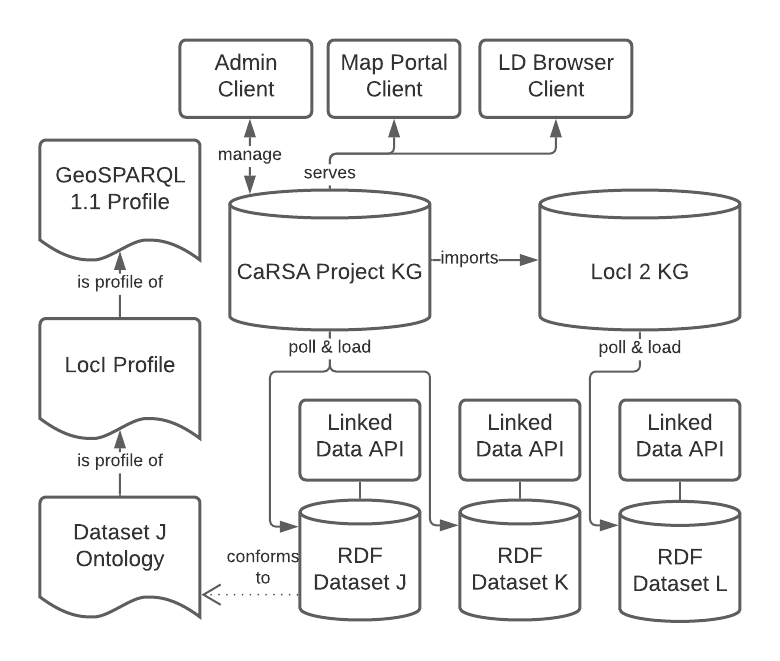
\includegraphics[width=0.8\linewidth]{images/carsa-arch.png}
    \caption{An informal architecture diagram of the CaRSA project's \textit{Linked Data} infrastructure}
    \label{fig:carsa-arch}
\end{figure}


\section{Conclusions}\label{sec:conclusions}
This project is both reuser of LocI systems and an extender of them. Core benefits of spatial Linked Data are preserved - distributed dataset publication, human- and machine-readable 
web content - and Semantic Web methods - inferencing, ontology modelling however new spatial data indexing is applied (Discrete Global Grid System use), total project data holdings management is
enabled, data validators created and new clients are delivered.


\subsection{Future Work}\label{sec:futurework}
This project will operate in test mode until July, 2021, after which time it is expected the system will move to full production. When that happens, this system will be highly dependent on the 
dependable supply of its datasets to make guarentees about system data currency. To ensure this, inter-agency data supply chain management - stated under the precursor LocI project but not completed - 
must be completed. 

For data to be delivered by owner agencies as Linked Data, assistance will need to be given to those agncies to be able to model datasets using Semantic Web ontologies and to produce Linked Data verisions
of them for delivery via APIs. This will require strong motivation from central government data users to ensure thee requriements are met as implementing these approaches and tools is a socio-technical
challenge, not purely a technical one.


%
% ---- Bibliography ----
%
% BibTeX users should specify bibliography style 'splncs04'.
% References will then be sorted and formatted in the correct style.
%
\bibliographystyle{splncs04}
\bibliography{references}
%
% \begin{thebibliography}{8}
% \bibitem{ref_article1}
% Author, F.: Article title. Journal \textbf{2}(5), 99--110 (2016)

% \bibitem{ref_lncs1}
% Author, F., Author, S.: Title of a proceedings paper. In: Editor,
% F., Editor, S. (eds.) CONFERENCE 2016, LNCS, vol. 9999, pp. 1--13.
% Springer, Heidelberg (2016). \doi{10.10007/1234567890}

% \bibitem{ref_book1}
% Author, F., Author, S., Author, T.: Book title. 2nd edn. Publisher,
% Location (1999)

% \bibitem{ref_proc1}
% Author, A.-B.: Contribution title. In: 9th International Proceedings
% on Proceedings, pp. 1--2. Publisher, Location (2010)

% \bibitem{ref_url1}
% LNCS Homepage, \url{http://www.springer.com/lncs}. Last accessed 4
% Oct 2017
% \end{thebibliography}
\end{document}




% Outline
% 
% Section 1
%   History of GeoSPARWL 1.0
% Section 2
%   motivation to update the spec
% Section 3
%   GeoSPARQL 1.1 additions
%       motivation, and expected use, of new spatial functions. In particular, why in GeoSPARQL when aggregations etc. can be performed elsewhere?
%       Spatial Measure
% Section 4
%       new profile presentation
%       new URI regimes etc
% Section 5
%       expected changed use modes